\documentclass[fontset = none]{ctexart}
\ctexset{fontset = fandol}
\author{\CJKfontspec{KaiTi} xzx}
\title{assignment1我的答案}
\usepackage{graphicx}


\begin{document}
\maketitle
\setcounter{page}{0}
\thispagestyle{empty}
\newpage

\section{Q1: k-Nearest Neighbor classifier}

\subsection{cs231n/classifier/k\_nearest\_neighbor.py}
\subsubsection{compute\_distances\_two\_loops(self,X) }
直接想比较困难,题目给出提示说将其转化为矩阵相乘以及两个和的形式。于是
想到将平方和展开。\\
为方便起见,先用平方距离进行计算,计算完成以后再将其开方。设两个向量为
W与V。那么这两个向量的平方距离应该为 $(w_1 - v_1)^2 + ... + (w_n-v_n)^2$
将起展开,得到 $x_1^2-2x_{1}y_1+y_1^2 + ... +x_n^2-2x_{n}y_n+y_n^2$,
继续变形,得:
$$\sum_{i=1}^{n}{x_i^2} +
\sum_{i=1}^{n}{y_i^2} -2\sum_{i=1}^n{x_{i}y_i}$$
这个式子的前两项就是题目中说的两个和的形式,后一项就是矩阵相乘的形式.

\section{Q2: Training a Support Vector Machine}

\subsection{cs231n/classifier/linear\_svm.py}
\subsubsection{svm\_loss\_vectorized(W, X, y, reg)}
\paragraph{loss}
首先把loss function的公式给列出来:
 $L_i = \sum_{j\neq y_i}max(0, s_j - s_{y_i} + 1)$
不管怎么样,肯定是要知道每一个图片对应的每一类的概率.先用$X * W$把分数算出来。\\
然后取出正确的分类的分数,相减.python中对于矩阵减去向量,
如果维数正确的话,它会自动补齐的.然后再加上 $\delta$,
最后把负数全部都变成0就好了.
\paragraph{微分}
首先不考虑要除以的num\_train。\\
首先看公式中 $s_j$ 与 $s_{y_i}$ 对loss的影响。当 $s_j - s_{y_i} + 1$ 小于0的时候,
对loss是没有影响的。当大于0的时候,如果 $s_j$ 变化1,则loss相应的变化1;如果 $s_{y_i}$
变化1,loss相应的变化-1. 这样, $ds$ 就可以表示出来了.\\
再来考虑每一个 $s_i,j$ 是怎么来的。假设说 $X$ 是 $(N,D)$ 的矩阵,$N$ 表示数据的个数, $D$ 表示
每个数据的维度, $W$ 是 $(D,C)$ 的矩阵, $C$ 表示类型的个数. $s_{i,j} = X_{[i,:]} * W_{[:,j]}$.
如果 $W_{[t,j]}$ 变化了1,则 $s_{i,j}$ 相应要变化 $X_{[i,t]}$ . 所以, $dW_{t,j}$ 就等于
$ds_{i,j} * X_{i,t}$ ,剩下的就是将起向量化就可以了。
下图以2维为例,描述了反向传播的过程
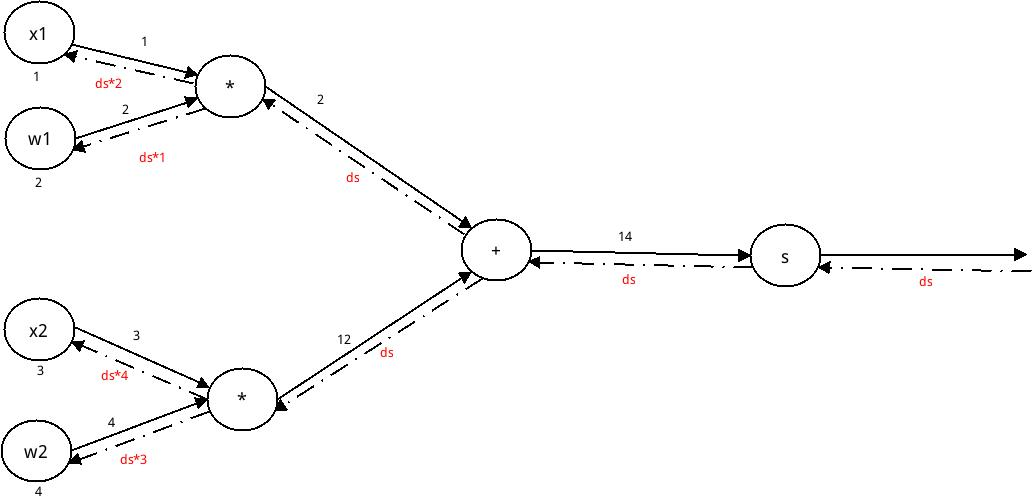
\includegraphics[width=5in]{./assignment1_pic/svm_loss_vectorized.jpg}
当然W会对不同的X乘很多次。对于W不同的分支来说,就是不同位置导数相加就是一个W的导数.

\subsection{Stochastic Gradient Descent}
这个函数没有什么难度,设计这个算法的思路就是因为Gradient\ Descent在大的数据集上太慢了,
就用了这么一个函数,每次随机选取几个数据进行Gradient\ Descent.


\section{Q3: Implement a Softmax classifier}
\subsection{cs231n/classifiers/softmax.py}
\subsubsection{softmax\_loss}
\paragraph{loss}
用$X$和前面算出来的$W$算出一个分数。还是假设只有一个数据,那算出来的分数就是这个数据对应
的每个类的分数,记为$s_j$.把这个数据分到第k类的概率是$\frac{e^{s_k}}{\sum_j{e^{s_j}}}$。
将正确的标签对应的概率取负对数就是需要的答案.loss没有什么可说的,反正naive跟vectorized都
一样。
\paragraph{微分}
先来看一下loss函数对于每一个$s_j$的导数.\\
假设正确的标记是y.损失函数用L来表示.即$L=-\log{\frac{e^{s_y}}{\sum_j{e^{s_j}}}}=
-(\log{e^{s_y}} - \log{\sum_j e^{s_j}}) = -s_y + \log{\sum_j e^{s_j}}$.\\
对$s_y$求导,$\frac{\partial L}{\partial s_y}=-1+\frac{e^{s_y}}{\sum_j{e^{s_j}}}$
对剩下的$s_k$求导,$\frac{\partial L}{\partial s_{k \neq y}} =
\frac{e^{s_k}}{\sum_j{e^{s_j}}}$\\
这样,ds就求出来了,剩下的就跟前面svm的地方反向传播一样就好了.







\end{document}
